\documentclass{article}
\usepackage{tikz}
\usepackage{amsmath}

\begin{document}

\section*{Propiedades sobre redes}

\begin{enumerate}
    \item Para cada una de las siguientes sentencias sobre el problema de flujo máximo en una red \( N \):
    \begin{enumerate}
        \item \textit{Si la capacidad de cada arista de \( N \) es par, entonces el valor del flujo máximo es par.}
        
        \textbf{Verdadero.} Sabemos que el flujo máximo en \( N \) es igual a la capacidad del corte mínimo. Como \( N \) tiene capacidades pares, todo corte de \( N \) tendrá capacidad par también, incluyendo naturalmente al corte mínimo. Luego, se sigue que el flujo máximo debe ser par.
        
        \item \textit{Si la capacidad de cada arista de \( N \) es par, entonces existe un flujo máximo en el cual el flujo sobre cada arista de \( N \) es par.}
        
        \textbf{Verdadero.} 
		Para demostrarlo usaremos la siguiente propiedad: \\
		 
        \textbf{Dada una red con capacidades todas pares, si dividimos a todas las capacidades de la red por 2, entonces el flujo maximo de la red original es igual a multiplicar por 2 el flujo maximo de la nueva red} \\
        
        \textbf{Demostracion:} Sabemos que el flujo maximo es igual al corte minimo, y la cantidad de cortes es finita. Lugo podemos ordenarlos por capacidades como :
        \[ C_1 \le C_2 \le \dots \le C_n\]
         Sabemos que como todas las capacidades en la red son pares, entonces las capacidades de $C_i$ es par $\forall 1 \le i \le n$
         Entonces podemos dividirlas en dos. Sea $C'_i = \frac{C_i}{2}$  y N² la red resultante de dividir a todas las capacidades en 2. Es claro que la relacion de orden entre las capacidades del los cortes no cambia al dividir a todas por 2, es decir
         \[ C'_1 \le C'_2 \le \dots \le C'_n\]
         
         Luego el flujo maximo en nuestro nuevo grafo N² es $C'_1$, que puede ser dado con algun flujo valido sobre la red.
         Pero recordemos que $C'_1*2 = C'_1$ , demostrando lo que queriamos ver.   \\
        
        Podemos construir el flujo pedido con el siguiente algoritmo: 
        
        Tomamos todas las capacidades y las dividimos en dos. Ahora nuestras aristas tendran capacidad par o impar \textit{(en particular  con capacidad 1, esto solo ocurre si su capacidad original era 2)}. Usamos Ford-Fulkerson sobre este grafo. Luego sobre el flujo resultante , multiplicamos en 2 el resultado y las capacidades de todas las aristas, junto con el flujo que pasa a traves de ellas. Es claro que realizar esta operacion, no anula la validez del flujo enviado, ya que el principio de conservacion de flujo sigue valiendo, y ninguna arista tiene su capacidad excedida. Por la propiedad anterior, sabemos que tenemos ahora un flujo maximo, y como multiplicamos al flujo que pasa por cada arista por 2, entonces tenemos que todas ellas deben tener flujo par.
        
      
        \item \textit{Si la capacidad de cada arista de \( N \) es impar, entonces el valor del flujo máximo es impar.}
        
        \textbf{Falso.} El argumento del inciso (a) ya no vale si las capacidades son impares. Dependiendo de cómo se distribuya el flujo, el valor del flujo máximo puede ser par o impar. Se muestra en el dibujo un contraejemplo
        
        \item \textit{Si la capacidad de cada arista de \( N \) es impar, entonces existe un flujo máximo en el cual el flujo sobre cada arista de \( N \) es impar.}
        
        \textbf{Falso.} No se garantiza que exista un flujo máximo donde todas las aristas tengan flujo impar, incluso si las capacidades son impares. Puede haber configuraciones de flujo máximo donde algunas aristas tengan flujo par. Se muestra en el dibujo un contraejemplo
   

\begin{figure}[ht]
    \centering
    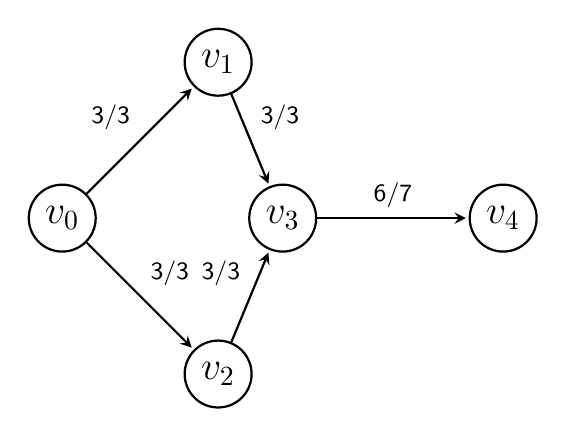
\begin{tikzpicture}[->,>=stealth,shorten >=1pt,auto,node distance=2.8cm,
                        thick,main node/.style={circle,draw,font=\sffamily\Large\bfseries}]
    
      \node[main node] (v0) {$v_0$};
      \node[main node] (v1) [above right of=v0] {$v_1$};
      \node[main node] (v2) [below right of=v0] {$v_2$};
      \node[main node] (v3) [right of=v0] {$v_3$};
      \node[main node] (v4) [right of=v3] {$v_4$};
    
      \path[every node/.style={font=\sffamily\small}]
        (v0) edge node {3/3} (v1)
             edge node {3/3} (v2)
        (v1) edge node {3/3} (v3)
        (v2) edge node {3/3} (v3)
        (v3) edge node {6/7} (v4);
    \end{tikzpicture}
    \caption{Contraejemplo de punto (c) y (d). A pesar de haber todas aristas con capacidades impares el flujo maximo es par, y no toda arista puede tener un flujo impar}
    \label{fig:flow_graph_redrawn}
\end{figure}

		\item \textit{Si todas las aristas de N tienen capacidades racionales, entonces el flujo máximo es racional.}
		
			\textbf{Verdadero.} Usamos el mismo argumento que el incisio (a). Todos los cortes tienen capacidad racional, luego el minimo tambien. Se sigue que el flujo maximo debe ser racional tambien.
\end{enumerate}
\end{enumerate}
\end{document}
